%!TEX root = ../dissertation.tex

\chapter{Tests and Results} \label{cha:test}

%%The purpose of this project is to show how a proto-AGI system such as OpenCog can be used 

\begin{table}[htbp]
  \centering
  \caption{Assemblable Objects Description Table}\label{Approcci}
  \medskip
\begin{tabular}{cccccccc}
\toprule
\multicolumn{4}{c}{\textbf{Assemblable Objects}} \\
\textbf{Number} &  \textbf{Quantity} &  \textbf{Colour} &  \textbf{Semantic Name}  \\
\midrule
\rowcolor{gray!35}
5 & 2 & Green/Orange & BearingSleeve1/BearingSleeve2 \\
6 & 1 & Blue & BettClamp \\
\rowcolor{gray!35}
7 & 1 & - & Bearing \\
9 & 2 & Grey/Gold & SnapRing1/SnapRing2 \\
\rowcolor{gray!35}
14 & 1 & - & TCEIScrew \\
31 & 1 & - & RotatingBalancerSupport \\
\rowcolor{gray!35}
32 & 1 & Red & RecirculatingBallSleeve \\
39 & 1 & - & UpperBearingBracket \\
\rowcolor{gray!35}
43 & 1 & Yellow & InductionHardenedRod \\
\bottomrule
\end{tabular}
\end{table}


\begin{figure} [h]
\centering
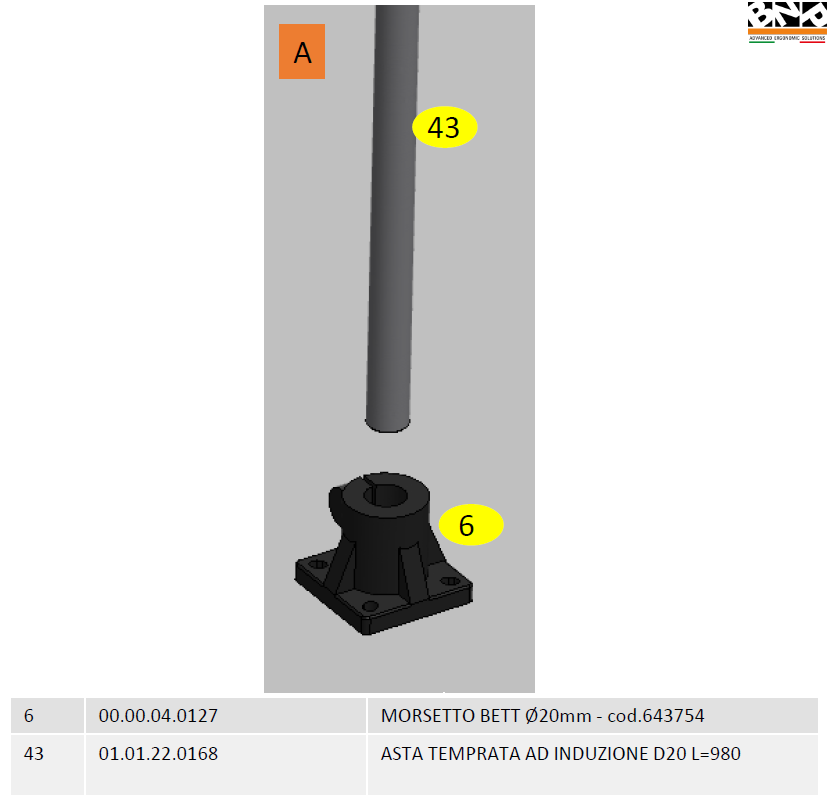
\includegraphics[width=1.0
\textwidth]{figures/Magistrale/ass_obj_1}
\caption[BFS Example]{
\label{fig:ass_obj_1}}
\end{figure} 

\begin{figure} [h]
\centering
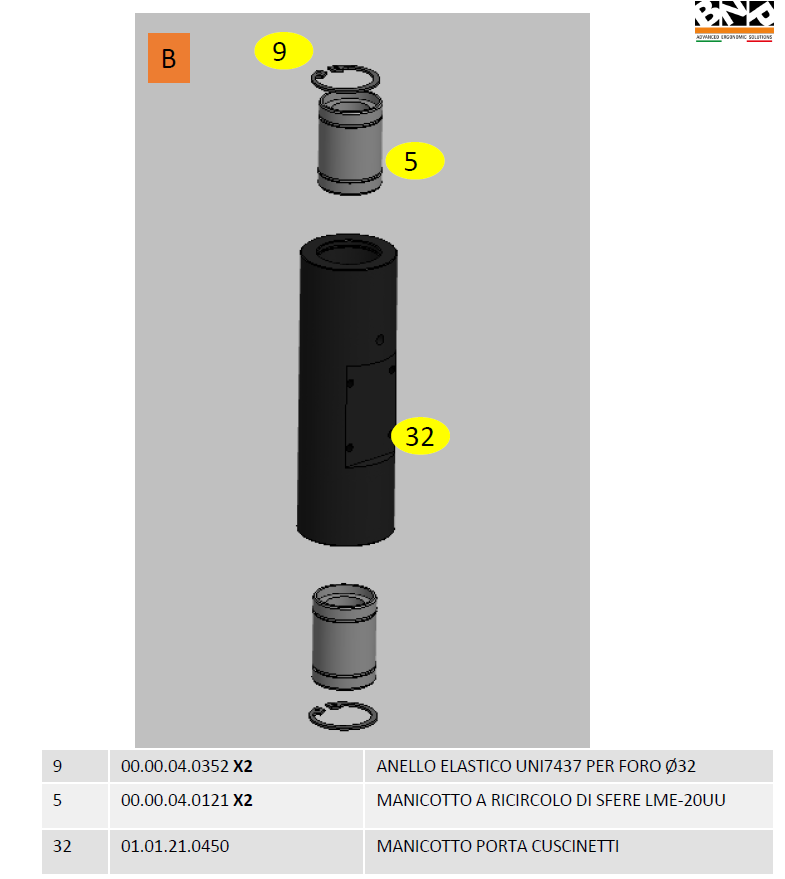
\includegraphics[width=1.0
\textwidth]{figures/Magistrale/ass_obj_2}
\caption[BFS Example]{
\label{fig:ass_obj_2}}
\end{figure} 

\begin{figure} [h]
\centering
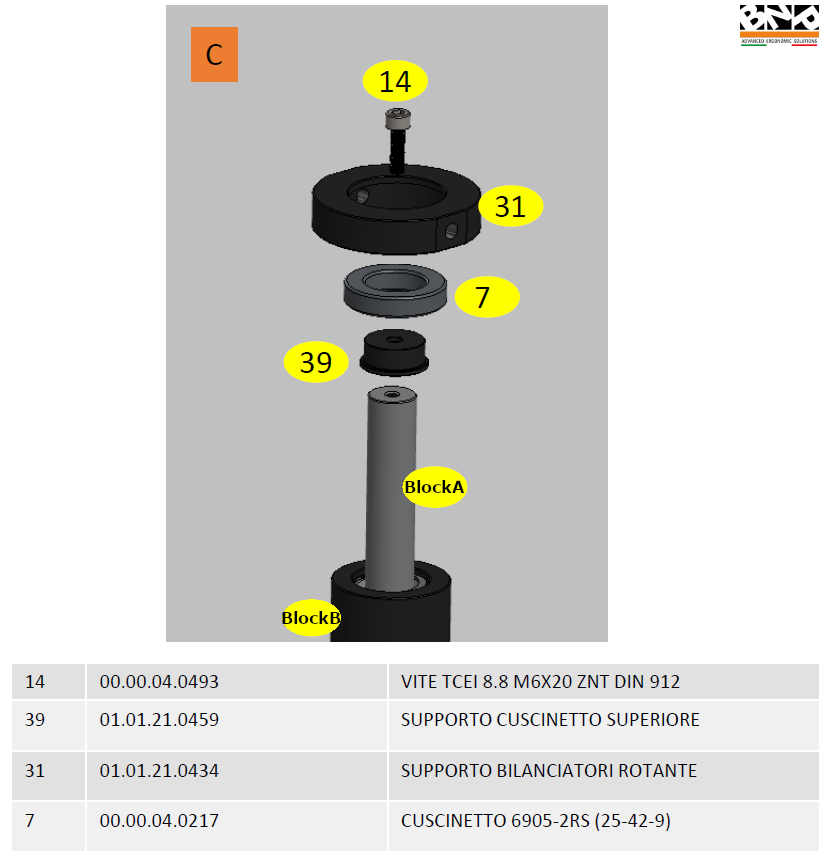
\includegraphics[width=1.0
\textwidth]{figures/Magistrale/ass_obj_3}
\caption[BFS Example]{
\label{fig:ass_obj_3}}
\end{figure} 